\documentclass[11pt,aspectratio=169]{beamer}
\usepackage[T1]{fontenc}
\usepackage[utf8]{inputenc}
\usepackage{lmodern,booktabs,array,textcomp}
\usepackage{graphicx}
\usepackage{tikz}
\usetikzlibrary{arrows.meta,positioning}
\newcommand{\euro}{\texteuro}

\definecolor{navy}{HTML}{0F1E2E}
\definecolor{navy2}{HTML}{14233a}
\definecolor{teal}{HTML}{0D8080}
\definecolor{tealbright}{HTML}{49dbc3}
\definecolor{ice}{HTML}{EEF5F5}
\definecolor{gold}{HTML}{C98A1B}
\definecolor{redish}{HTML}{B3414B}
\definecolor{violet}{HTML}{7857B8}

\usetheme{Madrid}
\usecolortheme{default}
\setbeamercolor{structure}{fg=teal}
\setbeamercolor{frametitle}{bg=navy,fg=white}
\setbeamercolor{title}{fg=navy}
\setbeamercolor{normal text}{fg=navy}
\setbeamercolor{footline}{fg=white,bg=navy}
\setbeamercolor{section in head/foot}{bg=navy,fg=white}
\setbeamercolor{author in head/foot}{bg=navy2,fg=white}
\setbeamercolor{title in head/foot}{bg=navy2,fg=white}
\setbeamercolor{block title}{bg=ice,fg=navy}
\setbeamercolor{block body}{bg=ice!40,fg=navy}
\setbeamercolor{alerted text}{fg=gold}
\setbeamertemplate{navigation symbols}{}
\setbeamertemplate{itemize items}[circle]
\newcommand{\code}[1]{\texttt{\detokenize{#1}}}

\title[Mini-IPHOREOS]{Mini-IPHOREOS}
\subtitle{From a Bayesian belief controller to a frozen, held-out evaluation \\ \small the Baseline system + four Extended-system milestones + the Transfer system}
\author{Florent Ouabo Kamkumo, PhD}
\date{4 October 2026}

\begin{document}

\begin{frame}
\begin{columns}
\begin{column}{0.52\textwidth}
\titlepage
\end{column}
\begin{column}{0.48\textwidth}
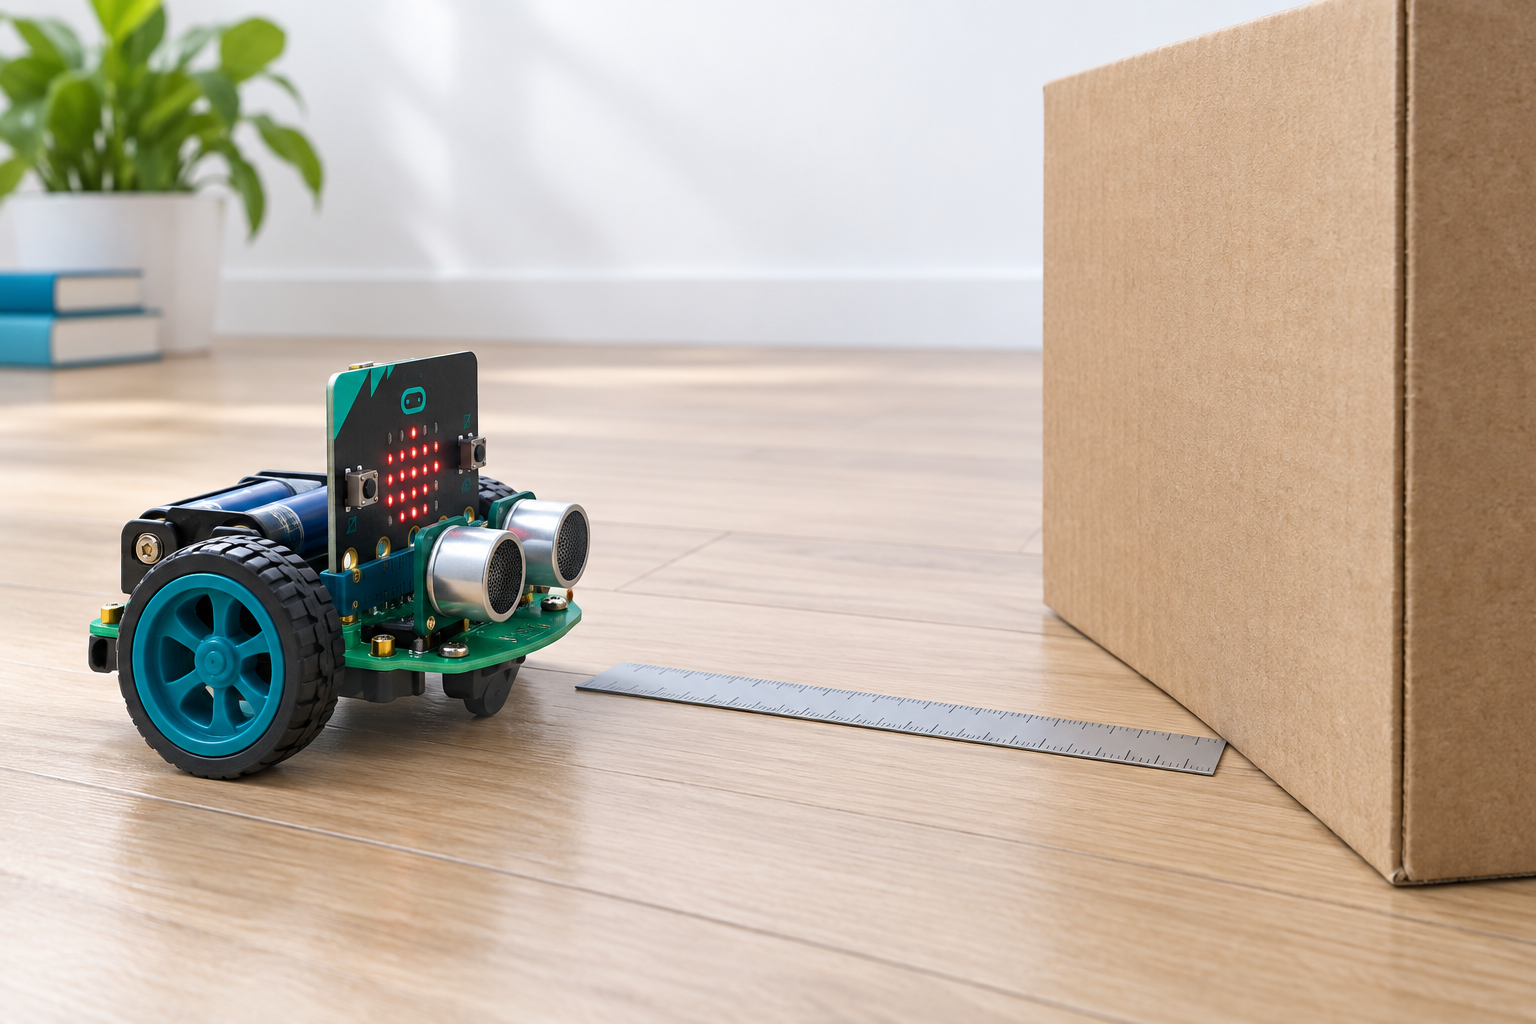
\includegraphics[width=\linewidth]{baseline_v1/assets/robot_concept.png}\\
{\tiny AI-generated concept illustration, not a photograph.}
\end{column}
\end{columns}
\end{frame}

\begin{frame}{What this talk covers}
\tableofcontents
\end{frame}

\section{What is Mini-IPHOREOS?}

\begin{frame}{The task, in one picture}
\begin{columns}
\begin{column}{0.55\textwidth}
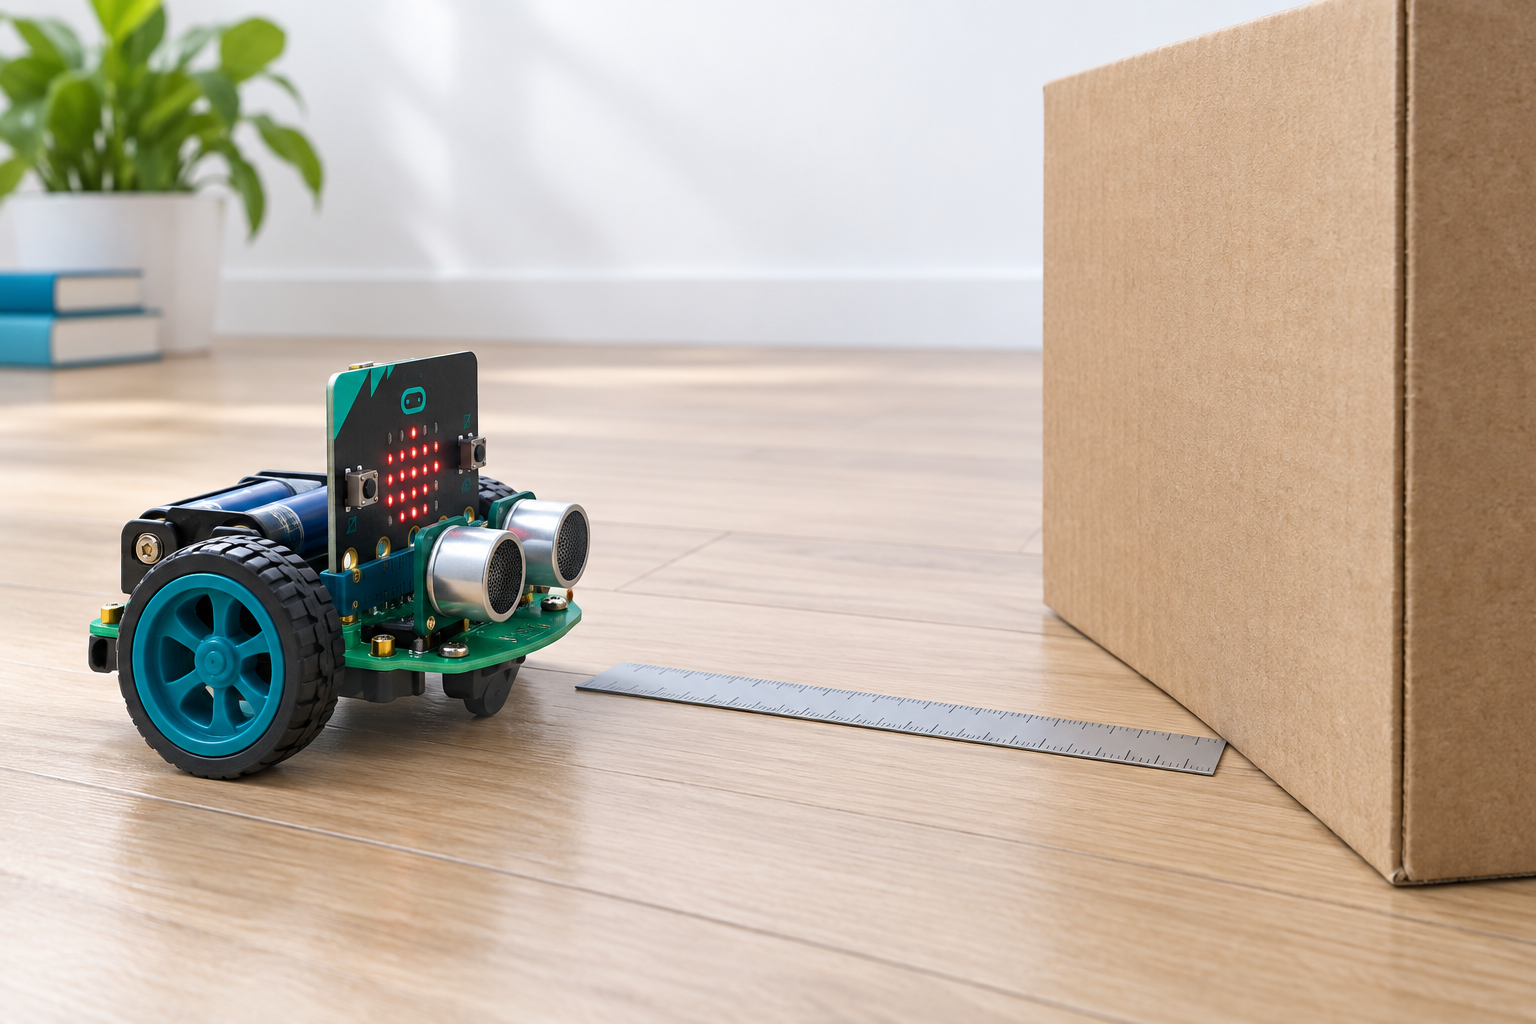
\includegraphics[width=\linewidth]{baseline_v1/assets/robot_concept.png}\\
{\tiny AI-generated concept illustration, not a photograph.}
\end{column}
\begin{column}{0.45\textwidth}
A small two-wheeled robot approaches a cardboard wall and must \textbf{stop with its sensor face 21--29\,cm away} (nominal target 25\,cm).
\begin{itemize}
\item Noisy ultrasonic distance readings
\item Imperfect, pulse-controlled motion
\item Must decide: move, measure, or stop and verify
\end{itemize}
\vspace{2mm}
\alert{Same observable task, from the first line of code to the last.} Every milestone below changes \emph{how the controller thinks}, never the task or the hardware interface.
\end{column}
\end{columns}
\end{frame}

\begin{frame}{IPHOREOS: concept -- event -- context -- policy}
\begin{itemize}
\item \textbf{Concept}: a goal state (``sensor face within band of the wall'')
\item \textbf{Event}: something observed or realised (a reading, a movement outcome)
\item \textbf{Context}: a hidden regime that shapes dynamics (surface speed, sensor bias)
\item \textbf{Policy}: a short sequence of actions chosen to make concepts come true
\end{itemize}
\vspace{4mm}
\begin{block}{What Mini-IPHOREOS actually is}
A reduced, rule-based demonstration of this idea, a disciplined Bayesian belief controller, \alert{not} a complete active-inference implementation. Two code lines: \code{baseline_v1} (the Baseline system) and \code{Mini_IPHOREOS_EXT1} (the Extended system), sharing the same sensor model and task.
\end{block}
\end{frame}

\section{The Baseline system}

\begin{frame}{The Baseline system: a scalar Bayesian belief}
\begin{columns}
\begin{column}{0.55\textwidth}
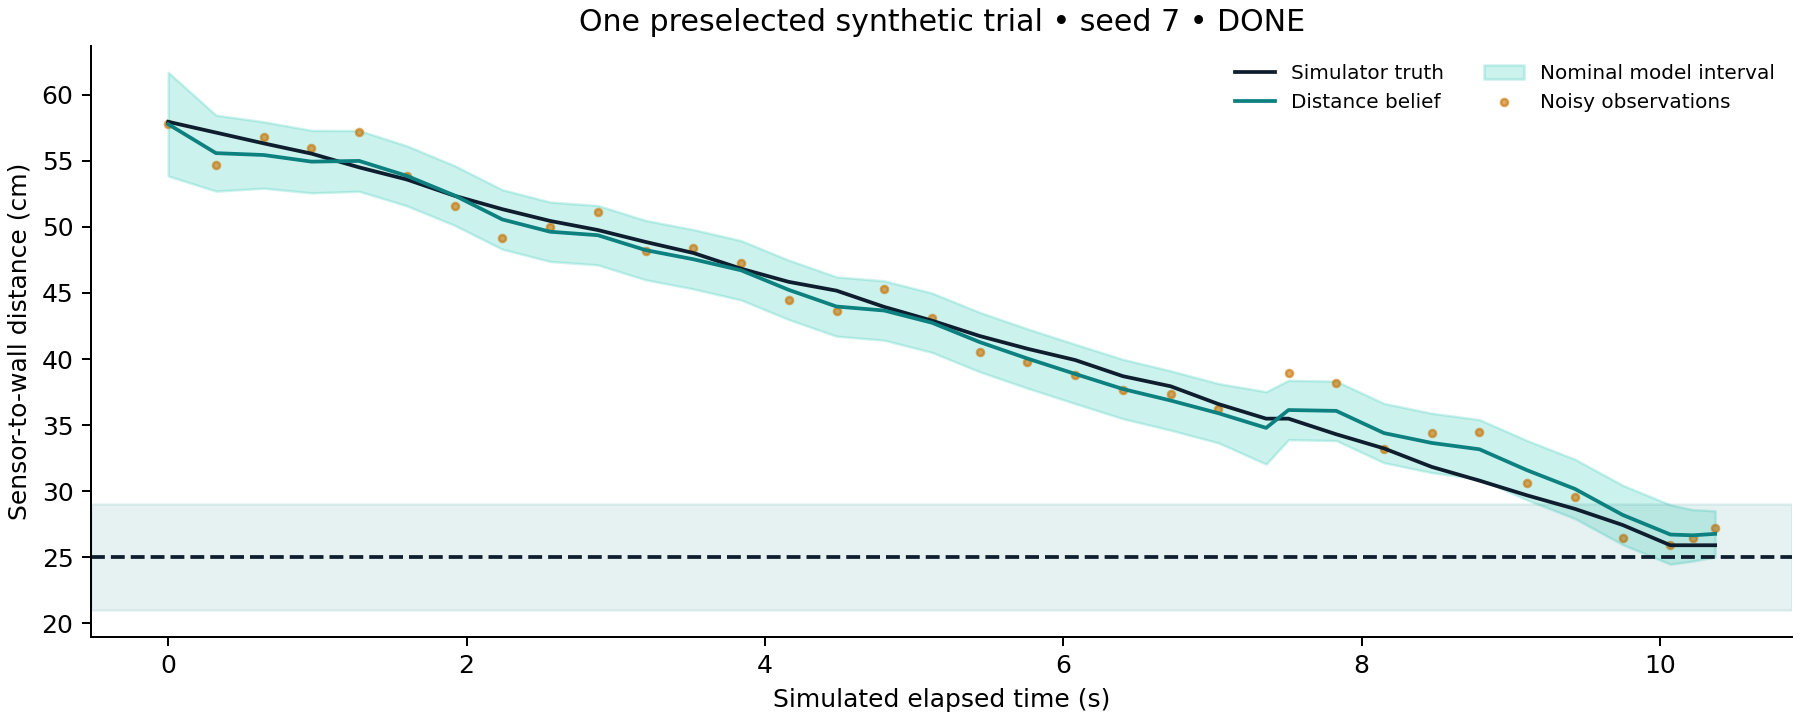
\includegraphics[width=\linewidth]{baseline_v1/assets/belief_trace.png}
\end{column}
\begin{column}{0.45\textwidth}
\begin{itemize}
\item One state: distance to the wall
\item Gaussian belief, updated from each noisy reading
\item A one-step rule: move, measure, or verify and stop
\item Three comparator policies: \textbf{Raw} (reading alone), \textbf{Belief} (Bayesian), \textbf{Mini} (Bayesian + verification band)
\end{itemize}
\vspace{2mm}
3{,}600 synthetic trials, computer-tested. \alert{No physical robot has run this code.}
\end{column}
\end{columns}
\end{frame}

\begin{frame}{The Baseline system's open problem: an unknown sensor bias}
\begin{columns}
\begin{column}{0.5\textwidth}
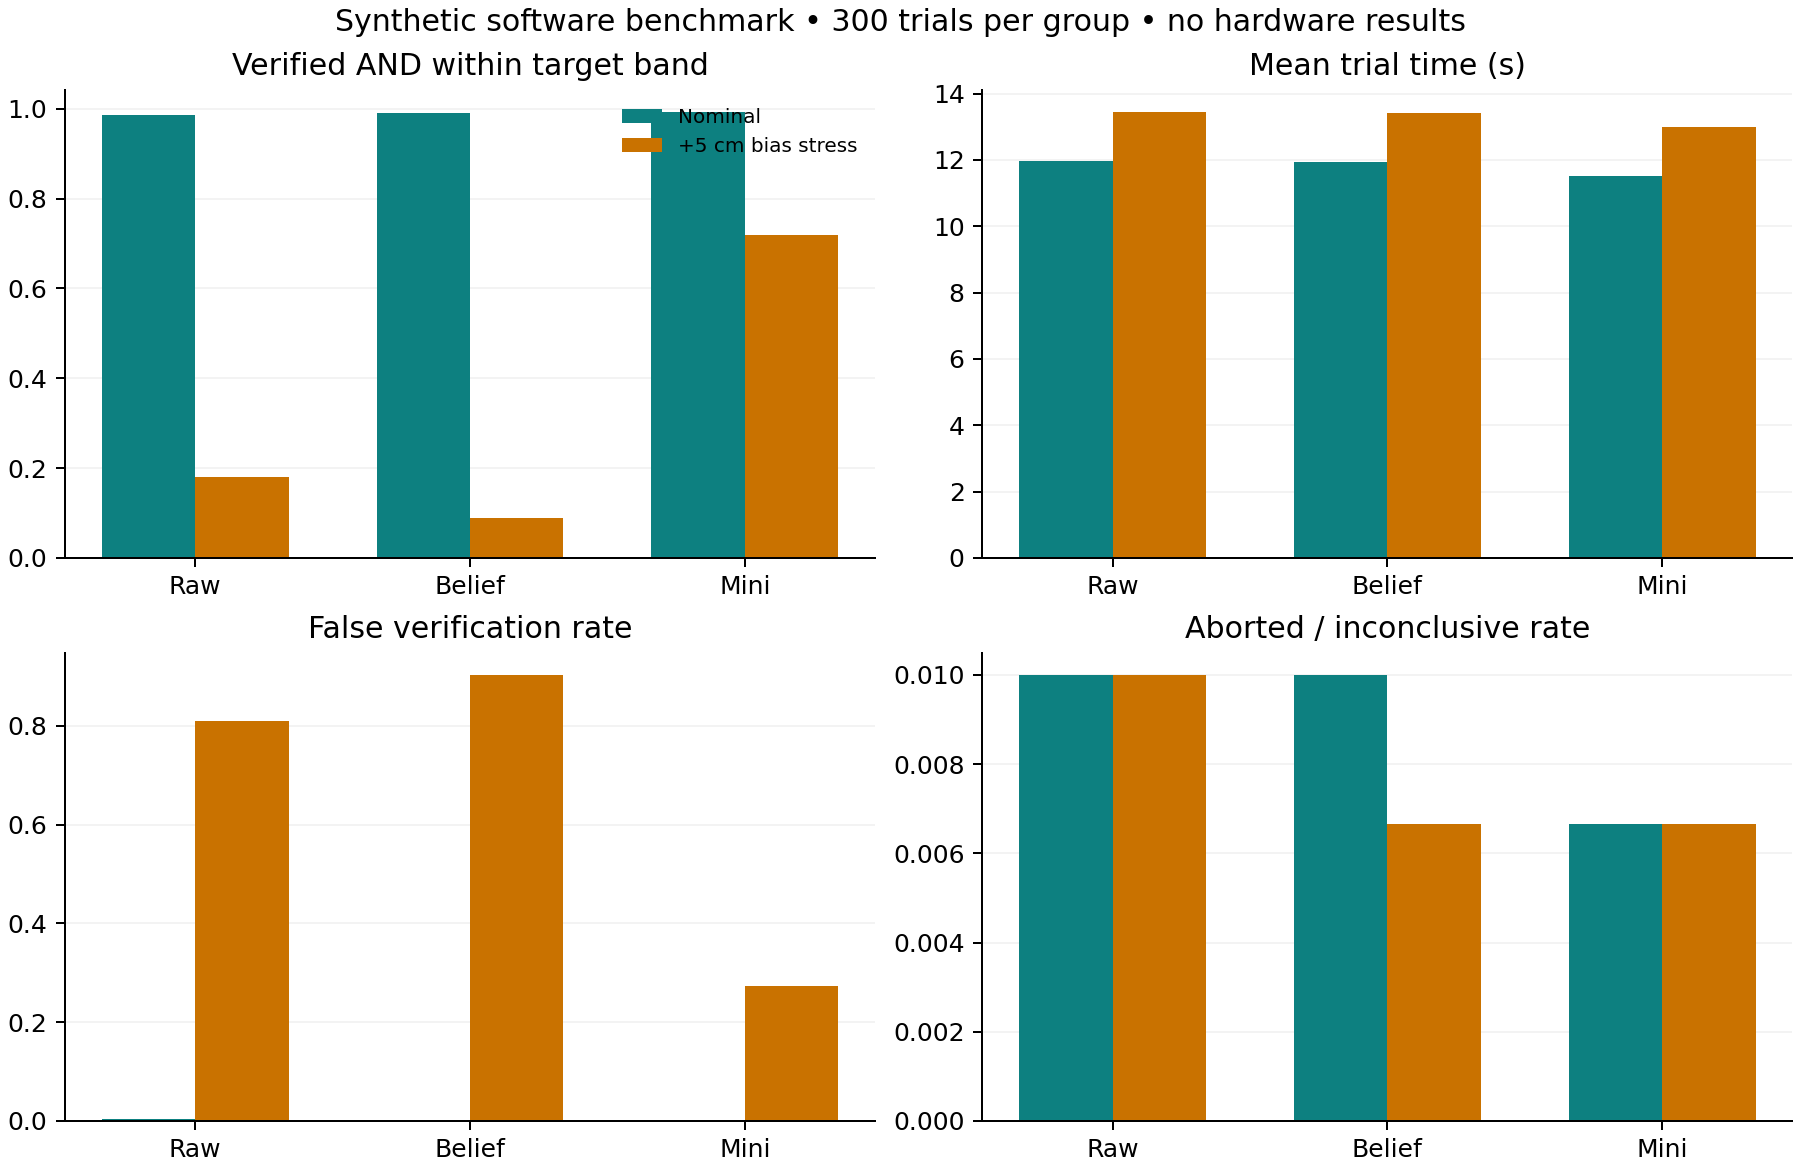
\includegraphics[width=\linewidth]{baseline_v1/assets/benchmark.png}
\end{column}
\begin{column}{0.5\textwidth}
Under a \textbf{+5\,cm constant sensor bias}, with no way to detect it:
\begin{itemize}
\item \textbf{Mini}'s verified-in-band rate falls from $\approx$0.99 to $\approx$0.72
\item its false-verification rate rises from $\approx$0 to $\approx$0.28
\end{itemize}
\vspace{3mm}
\alert{A confident, narrow belief is not the same as an accurate one.} This single finding motivates two of the Extended system's four milestones.
\end{column}
\end{columns}
\end{frame}

\section{The Extended system: a richer question}

\begin{frame}{The Extended system: four milestones, one six-item plan}
The Baseline system asks: \emph{given uncertain distance, move, measure, or stop?}\\
The Extended system asks: \emph{given uncertain distance \textbf{and speed}, under one of several possible contexts, what short sequence of actions best balances progress, cost, and the value of more information?}
\vspace{3mm}
\begin{block}{The original six-item improvement plan}
\begin{enumerate}
\item Fair, rule-based comparator baselines
\item A short-horizon (receding-horizon) planner
\item Context memory, so a recognised regime speeds up adaptation
\item A change-point detector, so memory is \emph{fast}, not just present
\item An explicit sensor-bias reference
\item A frozen, held-out evaluation
\end{enumerate}
\end{block}
\centering\alert{All six are now addressed, this talk walks through how.}
\end{frame}

\begin{frame}{The whole system, in one loop}
\begin{center}
\resizebox{0.72\linewidth}{!}{%
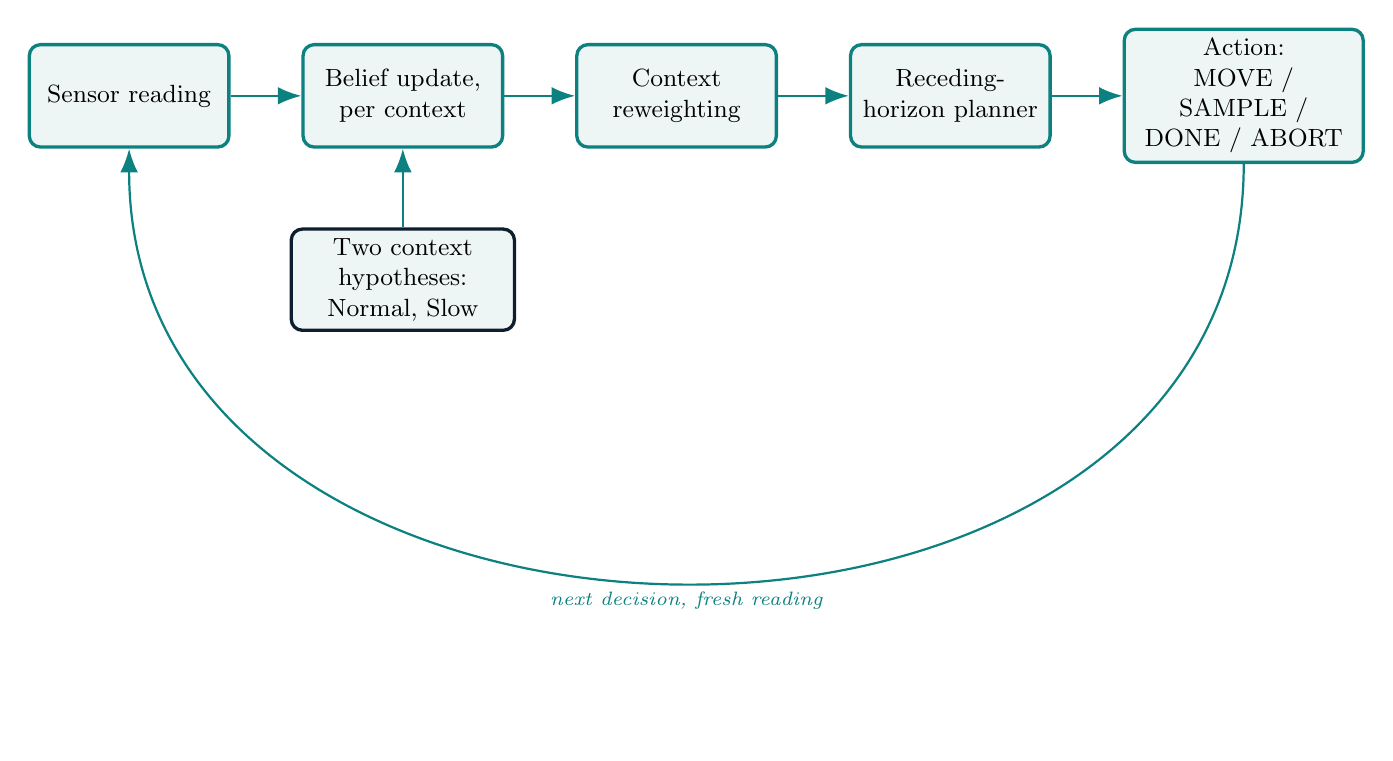
\begin{tikzpicture}[
  box/.style={rectangle,rounded corners,draw=teal,very thick,fill=ice,text width=2.3cm,align=center,minimum height=1.3cm,font=\small},
  hyp/.style={rectangle,rounded corners,draw=navy,very thick,fill=ice,text width=2.6cm,align=center,minimum height=1.1cm,font=\small},
  arr/.style={-{Latex[length=3mm]},thick,teal}
]
\node[box] (sensor) {Sensor reading};
\node[box,right=0.9cm of sensor] (update) {Belief update, per context};
\node[box,right=0.9cm of update] (reweight) {Context reweighting};
\node[box,right=0.9cm of reweight] (plan) {Receding-horizon planner};
\node[box,right=0.9cm of plan,text width=2.8cm] (action) {Action:\\MOVE / SAMPLE /\\DONE / ABORT};
\node[hyp,below=1cm of update] (hyp) {Two context hypotheses:\\Normal, Slow};
\draw[arr] (sensor) -- (update);
\draw[arr] (update) -- (reweight);
\draw[arr] (reweight) -- (plan);
\draw[arr] (plan) -- (action);
\draw[arr] (hyp) -- (update);
\draw[arr] (action.south) to[out=-90,in=-90,looseness=1.3] node[below,font=\scriptsize\itshape]{next decision, fresh reading} (sensor.south);
\end{tikzpicture}}
\end{center}
\vspace{2mm}
\centering\footnotesize One decision = one pass around this loop. Every milestone below changes one box or one arrow in it.
\end{frame}

\begin{frame}{What "two movement contexts" looks like}
\begin{center}
\resizebox{0.78\linewidth}{!}{%
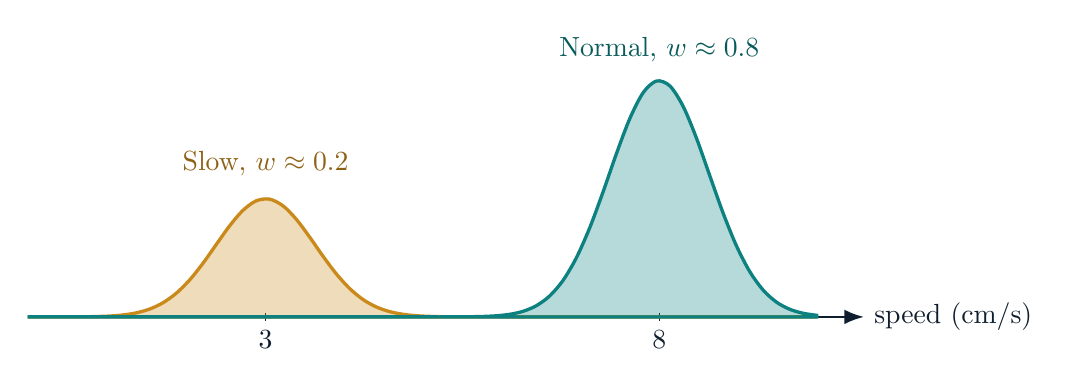
\begin{tikzpicture}
\draw[-{Latex[length=2.5mm]},thick,navy] (0,0) -- (10.6,0) node[right,font=\normalsize]{speed (cm/s)};
\draw[navy] (3,0.05) -- (3,-0.05) node[below,font=\normalsize]{3};
\draw[navy] (8,0.05) -- (8,-0.05) node[below,font=\normalsize]{8};
\draw[gold,very thick,fill=gold,fill opacity=0.3,domain=0:10,samples=60,smooth]
  plot ({\x},{1.5*exp(-((\x-3)*(\x-3))/0.8)}) -- (10,0) -- (0,0) -- cycle;
\draw[teal,very thick,fill=teal,fill opacity=0.3,domain=0:10,samples=60,smooth]
  plot ({\x},{3.0*exp(-((\x-8)*(\x-8))/0.8)}) -- (10,0) -- (0,0) -- cycle;
\node[gold!70!black,font=\normalsize] at (3,1.95) {Slow, $w\approx0.2$};
\node[teal!70!black,font=\normalsize] at (8,3.4) {Normal, $w\approx0.8$};
\end{tikzpicture}}
\end{center}
\vspace{3mm}
\centering Two running speed guesses held at once -- sketch only, not to calibrated scale. As readings arrive, whichever guess predicts them better wins weight.
\end{frame}

\section{Milestone 1: fair baselines + a planner that doesn't stall}

\begin{frame}{Milestone 1: a two-step planner, scored honestly}
\begin{columns}
\begin{column}{0.55\textwidth}
\includegraphics[width=\linewidth]{Mini_IPHOREOS_EXT1_Video/preview_EN_80s.png}
\end{column}
\begin{column}{0.45\textwidth}
\begin{itemize}
\item Joint (distance, speed) belief, two-mode mixture
\item Two-step receding-horizon planner with an explicit \textbf{no-progress cost}
\item Fair comparator: \code{v1_fair}, a rule-based policy given the \emph{same} context information as the Extended system, not a strawman
\end{itemize}
\vspace{2mm}
Without the no-progress cost, a one-step planner can prefer \textsc{Measure} forever once near the target. The two-step horizon fixes this directly.
\end{column}
\end{columns}
\end{frame}

\begin{frame}{Milestone 1: what it bought}
\begin{itemize}
\item \code{v1_fair} roughly \textbf{halves} \code{v1}'s move count on the \code{normal} scenario (ratio $\approx$0.54), for the same success rate
\item No-information policies (\code{adaptive_no_information}, \code{ext1_no_information}) stay at \textbf{1.00 success} -- the historically riskiest combination (context-aware, no active information-seeking) no longer stalls or fails
\end{itemize}
\vspace{4mm}
\begin{block}{Still open after this milestone}
Context memory, a sensor-bias reference, and a held-out evaluation.
\end{block}
\end{frame}

\section{Milestone 2: context memory}

\begin{frame}{Milestone 2: a negative result, first}
\begin{block}{The hypothesis}
Once a regime (normal / slow) has been seen before, \emph{recognising} it again should let the controller adapt faster than re-estimating from scratch.
\end{block}
\begin{block}{Attempt 1, a persistent library (failed)}
Keep a running mean/variance per context, reuse it as a prior. Result: \alert{no measurable speed-up} on the 2nd, 3rd, ... visit to a regime. Tracing individual decisions (not guessing) found why: the library only changes the speed \emph{target}, not how fast the belief itself re-converges.
\end{block}
\end{frame}

\begin{frame}{Milestone 2: recognise, then reuse}
\begin{columns}
\begin{column}{0.58\textwidth}
\includegraphics[width=\linewidth]{Mini_IPHOREOS_EXT1_Video/preview_memory_EN_flash.png}
\end{column}
\begin{column}{0.42\textwidth}
\textbf{Attempt 2}: a CUSUM change-point detector flags ``this looks like a regime switch'' from accumulated evidence, then \textbf{jumps} the belief directly to the stored value for that context.
\vspace{3mm}
\begin{itemize}
\item 1st visit to a regime: \textbf{identical} to no-memory ($\approx$4.3 decisions)
\item 2nd+ visits: \textbf{3.2--3.3} vs \textbf{4.7--4.9} decisions to reconverge
\item and more reliable, not just faster
\end{itemize}
\end{column}
\end{columns}
\end{frame}

\section{Milestone 3: an explicit sensor-bias reference}

\begin{frame}{Milestone 3: breaking the distance/bias confound}
\begin{columns}
\begin{column}{0.55\textwidth}
\includegraphics[width=\linewidth]{Mini_IPHOREOS_EXT1_Video/preview_biasheldout_EN_20s.png}
\end{column}
\begin{column}{0.45\textwidth}
A constant sensor offset and a genuinely slower robot look \textbf{identical} from decisions alone: a confound the Baseline system's bias stress test exposed.
\vspace{2mm}
\textbf{The fix}: 5 readings at a \emph{known} 50\,cm distance, taken once before the real approach. \code{mean(readings) - 50cm} becomes the bias estimate, fed into every later observation.
\end{column}
\end{columns}
\end{frame}

\begin{frame}{Milestone 3: what it recovered}
\begin{columns}
\begin{column}{0.55\textwidth}
\includegraphics[width=\linewidth]{Mini_IPHOREOS_EXT1_Video/preview_biasheldout_EN_40s.png}
\end{column}
\begin{column}{0.45\textwidth}
\begin{tabular}{lcc}
\toprule
Scenario & \code{ext1} & \code{ext1_bias_ref} \\
\midrule
constant bias & 0.86 & \textbf{0.99} \\
random bias & 0.53 & \textbf{0.99} \\
\bottomrule
\end{tabular}
\vspace{3mm}

Bias estimate error: \textbf{0.42\,cm} on average. Cost: 5 extra decisions, $\approx$0.75\,s, paid once per trial.
\end{column}
\end{columns}
\end{frame}

\section{Milestone 4: freeze it, then look at new data}

\begin{frame}{Milestone 4: the discipline}
\begin{alertblock}{Why this milestone exists}
Every number shown so far came from seeds 10000--10099, and several constants (CUSUM thresholds, library variances, jump weights, \code{REF_DISTANCE}, \code{N_REF}) were \emph{selected by grid search on that same range}. That is development-set reporting, not confirmation.
\end{alertblock}
\begin{itemize}
\item Every tunable constant frozen and written down \textbf{before} running anything further (\code{docs/FROZEN_PARAMETERS.md})
\item Full battery re-run, unmodified, on seeds \textbf{50000--50099}, never touched during three milestones of tuning
\item Plus one new test: an \textbf{outlier} scenario (corrupted-but-plausible readings), distinct from \code{dropout}'s missing readings
\end{itemize}
\end{frame}

\begin{frame}{Milestone 4: the new outlier scenario, reported honestly}
\begin{columns}
\begin{column}{0.55\textwidth}
\includegraphics[width=\linewidth]{Mini_IPHOREOS_EXT1_Video/preview_biasheldout_EN_glitch.png}
\end{column}
\begin{column}{0.45\textwidth}
A reading that is \emph{present} and in range, but badly wrong ($\pm$15--20\,cm). The innovation-rejection gate catches it.
\vspace{2mm}
Across 100 trials: most policies stay at \textbf{0.97--0.98} success.
\vspace{2mm}
\alert{\code{ext1_bias_ref} dips to 0.95} (abort 0.05 vs 0.02), its tighter post-calibration variance makes an unlucky \emph{first}-reading outlier costlier. Reported as a finding, not hidden.
\end{column}
\end{columns}
\end{frame}

\begin{frame}{Milestone 4: replication, dev seeds vs held-out seeds}
\small
\centering
\begin{tabular}{lcc}
\toprule
Claim & Dev (10000--10099) & Held-out (50000--50099) \\
\midrule
\code{v1_fair}/\code{v1} move ratio (normal) & 0.54 & 0.54 \\
No-information success & 1.00 & 1.00 \\
Memory+fast, 2nd+ visit (decisions) & 3.2--3.3 vs 4.6--4.9 & 3.2--3.3 vs 4.6--4.9 \\
Bias reference success (bias / random) & 0.86/0.53 $\to$ 0.99 & 0.78/0.52 $\to$ 1.00 \\
\bottomrule
\end{tabular}

\vspace{5mm}
\alert{Every headline claim replicates on data never used to tune anything.}
\end{frame}

\section{The full picture}

\begin{frame}{Nine policies, ten scenarios, one evaluation}
\centering
\includegraphics[width=0.92\linewidth]{results_ext1/comparison.png}
\vspace{2mm}

{\footnotesize All numbers from \code{results_ext1/summary.csv} and \code{results_ext1_heldout/}, produced by \code{experiments/run_simulation.py} and read (never asserted pass/fail) by \code{experiments/compare_heldout.py}.}
\end{frame}

\begin{frame}{Status}
\begin{block}{All six improvement-plan items are now addressed}
Fair baselines, the short-horizon planner, context memory with fast recognition, an explicit bias reference, and a frozen held-out evaluation, each implemented, tested, and verified against held-out data.
\end{block}
\begin{alertblock}{What ``status: addressed'' does \emph{not} mean}
\begin{itemize}
\item Not a claim that the model is a complete active-inference implementation
\item Not a claim that these numbers transfer to physical hardware
\item \textbf{Physical validation remains entirely separate and has not been attempted}
\end{itemize}
\end{alertblock}
\end{frame}

\section{Toward a physical experiment}

\begin{frame}{What transfers directly, and what does not}
\begin{itemize}
\item The sensor model, the motor-pulse mapping, and the task geometry: \textbf{shared} with the Baseline system's already-written physical tutorial (\code{baseline_v1/Tutorial_A_to_Z.pdf})
\item The Extended system's controller is plain NumPy, \textbf{incompatible} with MicroPython on the micro:bit as written
\item Two routes: (a) rewrite the belief/planner in MicroPython-safe arithmetic, or (b) run the Extended system on a companion host, with the micro:bit as a serial sensor/motor bridge
\end{itemize}
\vspace{3mm}
\begin{block}{Calibration that must be redone on hardware}
Per-context speed calibration, \emph{and} a physical version of the reference jig: a cut block or similar at a taped, ruler-verified 50\,cm.
\end{block}
\end{frame}

\begin{frame}{A staged test plan}
\begin{enumerate}
\item Stationary reference-jig checks: does the bias estimate match a ruler?
\item Supported-wheel motor checks (wheels off the ground): pulse-to-distance calibration
\item Single-controller floor trials: does the Baseline system's own task still verify correctly?
\item Context-memory trials: alternate two physical surfaces/speeds, check reconvergence
\item Bias-reference trials: deliberately offset the sensor, check recovery
\item A frozen-parameter physical campaign: same constants as the desktop evaluation, no tuning on physical data
\end{enumerate}
\vspace{2mm}
\centering{\footnotesize Full detail: \code{Tutorial_EXT1_EN.pdf}, Section 10.}
\end{frame}

\section{What to buy}

\begin{frame}{What to buy: the complete ensemble}
The Extended system needs nothing beyond the Baseline system's own build, plus a reference jig (a cut block or similar effectively free).

\vspace{2mm}
\small
\centering
\begin{tabular}{lrl}
\toprule
Item & Budget & Notes \\
\midrule
Kitronik :MOVE Motor \textbf{5683} & \euro{}44.38 & RS Germany listing incl. VAT \\
BBC micro:bit V2.21 Go Bundle & \euro{}18.90 & BerryBase listing incl. VAT \\
Four matched alkaline AA cells & \euro{}5.00 & Planning allowance \\
Ruler or tape measure & \euro{}5.00 & Planning allowance \\
Removable floor tape & \euro{}4.00 & Planning allowance \\
Broad cardboard target & \euro{}0.00 & Reuse a packaging box \\
Laptop and USB data cable & \euro{}0.00 & Existing equipment \\
Delivery across suppliers & \euro{}15.00 & Checkout-specific \\
Price/replacement reserve & \euro{}15.00 & Retained \\
\midrule
\textbf{Total planned envelope} & \textbf{\euro{}107.28} & Unspent reserve remains yours \\
\bottomrule
\end{tabular}
\end{frame}

\begin{frame}{Buying it correctly}
\begin{alertblock}{Buy exactly \textbf{:MOVE Motor 5683}}
Not :MOVE mini, a Maqueen, or a Raspberry Pi Pico buggy, similar names do not imply the same motor driver or pin mapping.
\end{alertblock}
\begin{itemize}
\item No purchase has been made as of this deck; prices must be reconfirmed at checkout
\item Full sourcing links and alternative suppliers: \code{baseline_v1/Tutorial_A_to_Z.pdf}, chapter 03
\item Assembly, wiring, and physical calibration: \code{baseline_v1/Tutorial_A_to_Z.pdf} directly, this project does not duplicate or change the Baseline system's motor programs
\end{itemize}
\end{frame}

\section{The Transfer system: a cross-task test of O3}

\begin{frame}{A later, separate question: does the library transfer to a new goal?}
\begin{block}{The question (Objective O3: ``recompose shared representations for a new goal'')}
Milestone 2's library speeds up reuse \emph{within} one task, across repeat visits. Does the \emph{same learned library} transfer \emph{across} tasks -- a genuinely different goal?
\end{block}
\textbf{Task B}: a second approach, target 85\,cm (band 81--89\,cm), start 115--145\,cm -- same sensor, same motor model, same normal/slow regimes as Task A; only the goal differs.
\begin{block}{Attempt 1, transfer the library as-is (failed)}
Train on Task~A, seed the learned library into Task~B three ways (cold start / zero-update transfer / adapt with updates). Result: \alert{no measurable difference, any condition, any metric}. Traced cause: the checkpoint learned speeds within noise of the plain calibration prior a cold-start belief already uses -- Task~A's training scenario draws from exactly those same calibration constants. Nothing to transfer, not a failure to transfer.
\end{block}
\end{frame}

\begin{frame}{Attempt 2: give it something calibration can't already supply}
\begin{columns}
\begin{column}{0.5\textwidth}
Each of the 100 standard seeds becomes its own \textbf{deployment}: a persistent $0.6$--$0.85\times$ speed bias, shared between that deployment's Task~A training and Task~B test, invisible to static calibration.
\vspace{2mm}
\begin{itemize}
\item Cold start now faces a \alert{provably wrong} prior
\item A checkpoint trained on that deployment's Task~A should already know the correction
\end{itemize}
\end{column}
\begin{column}{0.5\textwidth}
\scriptsize
\begin{tabular}{p{3.1cm}r}
\toprule
Metric & Cold vs.\ transfer \\
\midrule
Success/moves/dec.-to-target & \alert{no diff.} \\
Reconverge, post-switch & 5.20 vs \textbf{3.79--3.85} \\
\bottomrule
\end{tabular}
\vspace{2mm}

Paired by deployment ($n{=}100$): transfer reconverges faster in \textbf{61}, ties in 32, slower in only \textbf{7}.
\end{column}
\end{columns}
\begin{alertblock}{Positive preliminary evidence for O3 -- with its actual scope}
The library transfers across a genuine change of goal, and speeds up exactly what Milestone 2 showed it could ever speed up -- \emph{recognising which regime is active} -- not overall task completion time. Both halves reported together, not the favourable one alone.
\end{alertblock}
\end{frame}

\begin{frame}{Where to go next}
\begin{itemize}
\item \code{Tutorial_EXT1_EN.pdf} -- the full LaTeX tutorial (Sections 1--11)
\item \code{Mathematical_Model_EXT1.pdf} -- every equation, every milestone, and the Transfer system
\item Three captioned videos: Milestone 1, Milestone 2, Milestones 3--4 (\code{Mini_IPHOREOS_EXT1_Video/})
\item \code{baseline_v1/Tutorial_A_to_Z.pdf} -- the physical build, start to finish
\end{itemize}
\vspace{6mm}
\centering{\Large Thank you.}
\end{frame}

\end{document}
